\chapter{Es, Air, Uap}\label{ch:g2:ice-water-steam}

Air yang sama yang berdenting di gelasmu sebagai bongkahan es
mengucur sebagai minuman dan naik dari panci sup sebagai kepulan
putih. Satu zat tunggal, tiga \emph{wujud}. Tahun lalu kita menonton
kehangatan mencairkan sebongkah es; tahun ini kita berkenalan dengan
ketiga wujud zat yang dapat diambil air.

\section{Tiga wujud air}

\begin{example}[Tempat tinggal tiap wujud]\label{ex:g2:ice-water-steam:where}
Air dapat berada dalam tiga \emph{wujud zat}. \emph{Padat}: es ---
bongkahan es, es menggantung di bawah atap, embun beku di rumput,
salju. Zat padat itu keras dan mempertahankan bentuknya. \emph{Cair}:
air yang mengucur --- hujan, sungai, laut, gelasmu. Zat cair mengalir
dan mengambil bentuk wadahnya. \emph{Gas}: uap air, yaitu air yang
terbang tanpa terlihat di udara. Padat, cair, gas --- tetapi selalu
zat yang sama di baliknya.
\end{example}

\begin{omfigure}
\begin{tikzpicture}[scale=0.85]
  \draw[thick, omDef] (0.3,0.1) rectangle (1.5,1.3);
  \node[below, font=\small] at (0.9,-0.2) {es: padat};
  \draw[thick] (3.9,1.5) -- (4.2,0.1) -- (5.6,0.1) -- (5.9,1.5);
  \fill[omDef, opacity=0.25] (4.13,0.45) -- (5.67,0.45)
    -- (5.75,1.1) -- (4.05,1.1) -- cycle;
  \node[below, font=\small] at (4.9,-0.2) {air: cair};
  \draw[thick] (8.0,0.1) rectangle (10.4,1.0);
  \draw[thick] (10.4,0.75) -- (11.0,0.85);
  \foreach \x/\y in {8.6/1.35, 9.2/1.7, 9.8/1.4, 9.0/2.05} {
    \draw[omExo, thick] (\x,\y) circle (0.22);
  }
  \node[below, font=\small] at (9.2,-0.2) {uap air: gas};
\end{tikzpicture}

{\small Tiga wujud satu zat: bongkahan es yang padat, segelas air yang
cair, dan kepulan di atas panci yang membocorkan adanya gas.}
\end{omfigure}

\begin{remark}[Uap air tidak terlihat]\label{rem:g2:ice-water-steam:invisible}
Kepulan putih yang kamu lihat di atas panci terbuat dari titik-titik
air mungil yang melayang --- tetes-tetes kecil zat \emph{cair}.
Gasnya yang sejati --- uap air yang bercampur ke dalam udara --- sama
sekali tidak dapat dilihat! Amati baik-baik cerat panci: tepat di
atasnya ada celah \emph{bening} yang pendek sebelum kepulan putih
dimulai. Di celah itu airnya berwujud gas, tidak terlihat; sedikit
lebih tinggi ia berkumpul menjadi tetes yang dapat kamu lihat. Uap air
yang tak terlihat bersembunyi di udara setiap ruangan, dan kita akan
menangkapnya sebelum bab ini berakhir.
\end{remark}

\begin{omfigure}
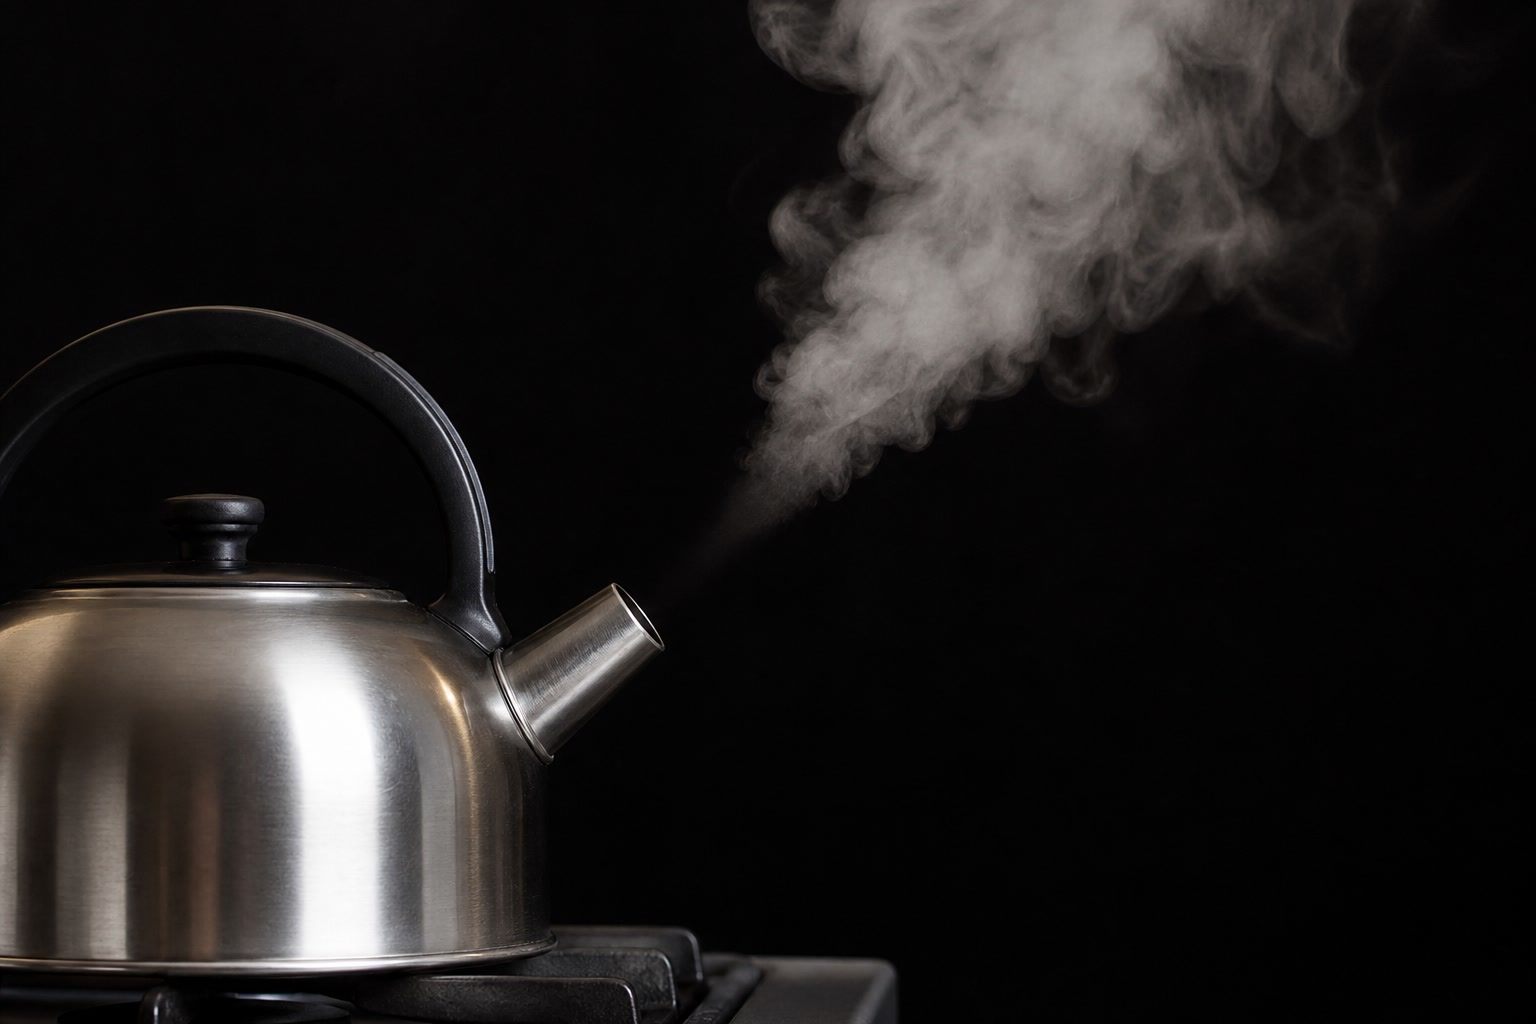
\includegraphics[width=0.55\linewidth]{images/book1/ai/g2-ice-water-steam-kettle.jpg}

{\small Rahasia cerek: tepat di atas cerat, ada celah \emph{bening} yang pendek tempat airnya berwujud gas tak terlihat --- baru lebih tinggi ia \omterm{def:g2:ice-water-steam:evapcond}{mengembun} menjadi kepulan putih yang dapat kita lihat.}
\end{omfigure}

\section{Berubah wujud}

\begin{definition}[Mencair dan membeku]\label{def:g2:ice-water-steam:meltfreeze}
Ketika kehangatan mengubah es yang padat menjadi air yang cair, es itu
\emph{mencair}\index{mencair}. Ketika dingin yang kuat mengubah air
yang cair menjadi padat, air itu \emph{membeku}\index{membeku}.
Mencair dan membeku adalah dua pintu berlawanan antara dua wujud yang
sama: kehangatan mendorong ke satu arah, dingin mendorong ke arah
sebaliknya.
\end{definition}

\begin{definition}[Menguap dan mengembun]\label{def:g2:ice-water-steam:evapcond}
Ketika kehangatan membuat air yang cair terbang ke udara sebagai gas,
air itu \emph{menguap}\index{menguap} --- genangan menyusut, cucian
mengering. Ketika uap air menyentuh benda yang dingin lalu berubah
kembali menjadi tetes cair, uap itu \emph{mengembun}\index{mengembun}
--- kabut pada jendela yang dingin, embun pada cermin kamar mandi.
Sekali lagi dua pintu berlawanan: kehangatan mengirim air ke wujud
gas, dingin memanggilnya kembali ke wujud cair.
\end{definition}

\begin{omfigure}
\begin{tikzpicture}[scale=0.85]
  \node[font=\small, draw, thick, omDef, minimum width=1.9cm,
    minimum height=0.85cm] (ice) at (0.8,0) {padat};
  \node[font=\small, draw, thick, omDef, minimum width=1.9cm,
    minimum height=0.85cm] (water) at (5.3,0) {cair};
  \node[font=\small, draw, thick, omDef, minimum width=1.9cm,
    minimum height=0.85cm] (steam) at (9.8,0) {gas};
  \draw[-Stealth, very thick, omThm] (1.85,0.28) -- (4.25,0.28);
  \node[above, font=\small, omThm] at (3.05,0.42) {kehangatan: mencair};
  \draw[-Stealth, very thick, omDef] (4.25,-0.28) -- (1.85,-0.28);
  \node[below, font=\small, omDef] at (3.05,-0.42) {dingin: membeku};
  \draw[-Stealth, very thick, omThm] (6.35,0.28) -- (8.75,0.28);
  \node[above, font=\small, omThm] at (7.55,0.42) {kehangatan: menguap};
  \draw[-Stealth, very thick, omDef] (8.75,-0.28) -- (6.35,-0.28);
  \node[below, font=\small, omDef] at (7.55,-0.42) {dingin: mengembun};
\end{tikzpicture}

{\small Perubahan wujud: kehangatan selalu mendorong ke kanan, dingin
selalu mendorong kembali ke kiri.}
\end{omfigure}

\begin{example}[Cobalah: tangkap air yang tak terlihat]\label{ex:g2:ice-water-steam:catch}
Ambillah sebuah kaleng atau gelas langsung dari lemari es, keringkan
bagian luarnya baik-baik dengan lap, lalu letakkan di atas meja.
Tunggulah sambil menghitung sampai $100$. Bagian luarnya menjadi
berkabut, lalu basah --- tetes air muncul entah dari mana! Tetes itu
tidak merembes lewat kaca: uap air yang tak terlihat di udara ruangan
menyentuh dinding yang dingin lalu \omterm{def:g2:ice-water-steam:evapcond}{mengembun}. Kamu baru saja menangkap
gas yang tak terlihat itu.
\end{example}

\begin{example}[Awan dari napas]\label{ex:g2:ice-water-steam:breath}
Napasmu selalu membawa uap air yang tak terlihat. Pada hari yang
hangat, uap itu tetap tak terlihat. Pada pagi yang membekukan, udara
luar yang dingin langsung mengembunkannya menjadi awan kecil di depan
mulutmu --- dan hal yang sama terjadi pada jendela yang dingin ketika
kamu mengembuskan napas untuk menggambar dengan jarimu.
\end{example}

\begin{remark}[Uap dan kompor: hati-hati]\label{rem:g2:ice-water-steam:safety}
Uap air di atas panci yang mendidih panas membakar --- lebih panas
daripada airnya sendiri terasa. Jangan pernah memasukkan tanganmu ke
dalam kepulan itu, dan angkatlah tutup panci menjauh dari tubuhmu,
dengan orang dewasa di dekatmu. Perubahan wujud untuk ditonton, bukan
untuk disentuh, setiap kali ada kompor yang terlibat.
\end{remark}

\section{Air yang sama, berputar-putar}

\begin{example}[Genangan yang menyusut]\label{ex:g2:ice-water-steam:puddle}
Sesudah hujan, sebuah genangan berkilau di halaman bermain. Menjelang
sore genangan itu sudah menyusut; besok ia sudah lenyap. Tidak ada
yang meminumnya dan ia tidak merembes lewat aspal: kehangatan Matahari
membuatnya \omterm{def:g2:ice-water-steam:evapcond}{menguap}, tetes demi tetes, ke udara. Gambarlah garis kapur
di sekeliling sebuah genangan pada pagi hari dan periksalah sesudah
makan siang: airnya sudah mundur ke dalam garismu.
\end{example}

\begin{example}[Dari laut sampai hujan]\label{ex:g2:ice-water-steam:cycle}
Apa yang \omterm{def:g2:ice-water-steam:evapcond}{menguap} pasti \omterm{def:g2:ice-water-steam:evapcond}{mengembun} di suatu tempat. Air terbang naik
dari laut dan genangan, tanpa terlihat; tinggi di langit, tempat
udaranya dingin, air itu \omterm{def:g2:ice-water-steam:evapcond}{mengembun} menjadi tetes-tetes yang membentuk
awan; tetes-tetes itu berkumpul, menjadi berat, lalu jatuh --- hujan!
Hujan mengisi genangan dan laut, dan perjalanan bolak-balik itu mulai
lagi. Air di gelasmu sudah menempuh perjalanan ini lebih sering
daripada yang dapat dihitung siapa pun.
\end{example}

\section{Latihan}

\begin{exercise}[$\star$]\label{exo:g2:ice-water-steam:1}
Wujud zat apa masing-masing benda ini --- padat, cair, atau gas: es
yang menggantung; \ laut; \ air tak terlihat tepat di atas cerat panci
sup; \ embun beku di rumput; \ hujan?
\end{exercise}

\begin{exercise}[$\star$]\label{exo:g2:ice-water-steam:2}
Sebutkan perubahan wujudnya: manusia salju yang menyusut di bawah
matahari; \ genangan yang lenyap; \ kabut yang muncul pada cermin kamar
mandi; \ kolam yang mengeras pada musim dingin.
\end{exercise}

\begin{exercise}[$\star$]\label{exo:g2:ice-water-steam:3}
Pada gambar perubahan wujud, ke arah mana kehangatan selalu
mendorong: ke wujud padat atau ke wujud gas? Dan dingin?
\end{exercise}

\begin{exercise}[$\star$]\label{exo:g2:ice-water-steam:4}
Tetes air pada kaleng dingin di \cref{ex:g2:ice-water-steam:catch} ---
apakah tetes itu merembes keluar lewat kaca? Dari mana asalnya?
\end{exercise}

\begin{exercise}[$\star$]\label{exo:g2:ice-water-steam:5}
Mengapa kamu dapat melihat napasmu pada pagi yang membekukan, tetapi
tidak pada hari yang hangat? Pakailah kata-kata pada
\cref{def:g2:ice-water-steam:evapcond}.
\end{exercise}

\begin{exercise}[$\star$]\label{exo:g2:ice-water-steam:6}
Cucian basah lebih cepat kering di bawah matahari daripada di tempat
teduh. Perubahan wujud mana yang bekerja, dan apa yang ditambahkan
Matahari untuk mempercepatnya?
\end{exercise}

\begin{exercise}[$\star$]\label{exo:g2:ice-water-steam:7}
Mengapa kepulan di atas panci yang mendidih berbahaya, dan apa aturan
amannya menurut \cref{rem:g2:ice-water-steam:safety}?
\end{exercise}

\begin{exercise}[$\star$]\label{exo:g2:ice-water-steam:8}
Ceritakan perjalanan bolak-balik setetes hujan: mulai dari laut,
berakhir kembali di laut, dan pakailah kata \omterm{def:g2:ice-water-steam:evapcond}{menguap} dan \omterm{def:g2:ice-water-steam:evapcond}{mengembun} di
sepanjang jalan.
\end{exercise}

\begin{exercise}[$\star\star$]\label{exo:g2:ice-water-steam:9}
Pada cerat panci ada celah bening, dan baru di atasnya kepulan putih
dimulai. Apa yang ada di celah bening itu? Apa yang ditunjukkannya
tentang air dalam wujud gas?
\end{exercise}

\begin{exercise}[$\star\star$]\label{exo:g2:ice-water-steam:10}
Nino meninggalkan segelas air di ambang jendela selama seminggu;
permukaannya turun hari demi hari, padahal tidak ada yang meminumnya.
Kucingnya dituduh. Belalah kucing itu: jelaskan apa yang sebenarnya
terjadi, dan ciptakan satu cara untuk menunjukkan bahwa airnya pergi
\emph{ke udara}, bukan ke dalam kucing.
\end{exercise}
